\documentclass{article}
\usepackage[utf8]{inputenc}
\usepackage{hyperref}
\usepackage{graphicx}
\setlength{\parskip}{1em}
\usepackage[margin=1.0in]{geometry}

\title{Lab 2: Getting to know the myRIO-1900 \\
  \large ECSE 421: Embedded Systems \\ Department of Electrical and Computer Engineering \\ McGill University \\ Version 1.1}
\author{Adam Cavatassi and Brett Meyer}
\date{Winter 2018}

\begin{document}

\maketitle

\section{Introduction}
In this lab, you will become acquainted with the myRIO development process. You will be required to set up and update the NI myRIO-1900 before you can continue with the rest of the labs in this course. Once you have ensured that your myRIO board is ready to be programmed, you will then make use of the accelerometer to practice data collection. All setup and lab instructions have been verified to work with LabVIEW 2016 on the PCs in Trottier Building Room 5090.

\section{Setting up the myRIO}
Once your board is plugged into your computer, a dialog should be automatically prompted to setup the board. A program called myRIO USB Monitor will be launched, as in Figure \ref{fig:s_1}. Your myRIO serial number and IP address should both be displayed at the top of the window. The IP address should be 172.22.11.2. Click \textbf{Launch the Getting Started Wizard} to proceed. 

\begin{figure}[h!]
\centering
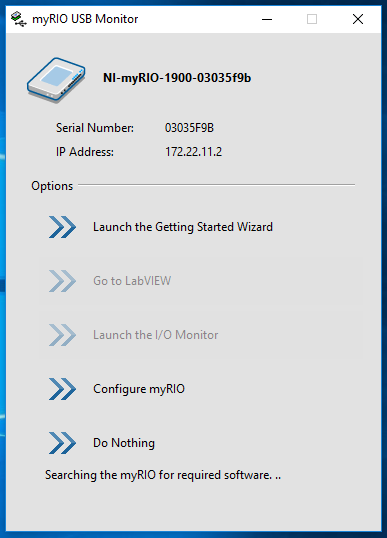
\includegraphics[scale=0.8]{figs/setup_1.png}
\caption{myRIO USB Monitor should automatically launch when your myRIO is connected.}
\label{fig:s_1}
\end{figure}

The next window will ask you to select a device to set up. It should look like Figure \ref{fig:s_2}. Select your myRIO to proceed. You will eventually be prompted to select a software to install on the myRIO board. Select LabVIEW 2016 and install it if it is not already. This will take 5 to 10 minutes. Once the installation is complete, you will be able to verify that all myRIO peripherals are functional. The test screen will allow you to check that the accelerometer, digital button, and output LEDs are working properly. You will notice that the Z-axis has an accelerometer reading of 1g (if your myRIO is laying flat on the table). Please ensure that all myRIO peripherals are working before proceeding any further. If you have an issue with your board, you will need to exchange it for a new one. Figure \ref{fig:s_3} is what the test window should look like. Once you have completed all these steps, you are ready to program the board in LabVIEW 2016. 


\begin{figure}[h!]
\hspace{25mm}
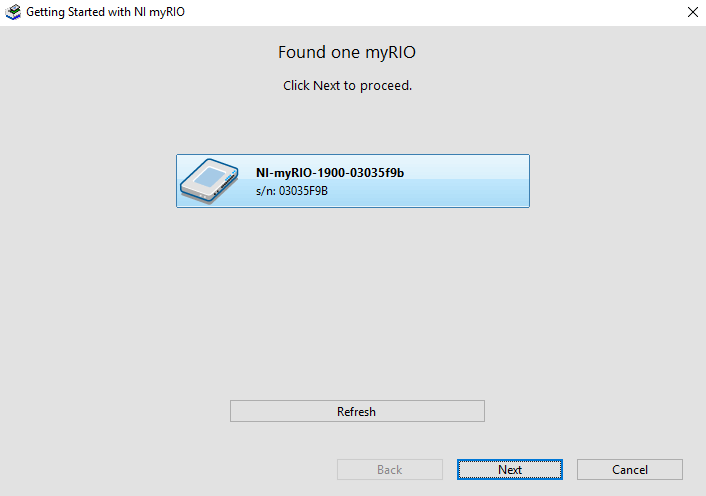
\includegraphics[scale=0.6]{figs/setup_2.png}
\caption{Select your device.}
\label{fig:s_2}
\end{figure}

\begin{figure}[h!]
\hspace{25mm} 
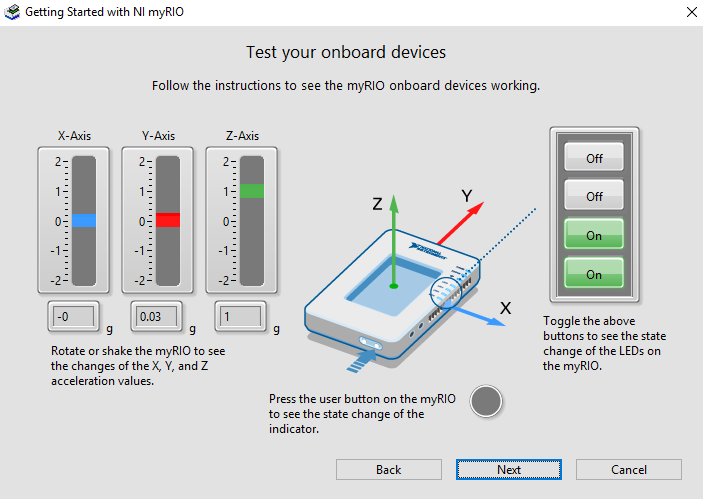
\includegraphics[scale=0.6]{figs/setup_3.png}
\caption{Test all myRIO peripherals.}
\label{fig:s_3}
\end{figure}

\section{Setting up a myRIO project}
For this lab, you will be writing a LabVIEW program that will run directly on the myRIO rather than on the PC as in the previous lab. You can begin by opening LabVIEW 2016 (32-bit) and creating a new blank project. Do not choose the myRIO template. Right click on \textbf{Project: \textless name of your project\textgreater} then go to \textbf{New}, then \textbf{Targets and Devices...}. The window that pops up should let your choose an existing device. Under the myRIO directory, your board should appear as in Figure \ref{fig:_2}. Once your board has been added as a target to your project, you can instantiate a new VI directly on the board. Right click your board (make sure than the IP address shows up beside the name of the board), go to \textbf{New}, select \textbf{VI}.

\begin{figure}[h!]
\hspace{25mm} 
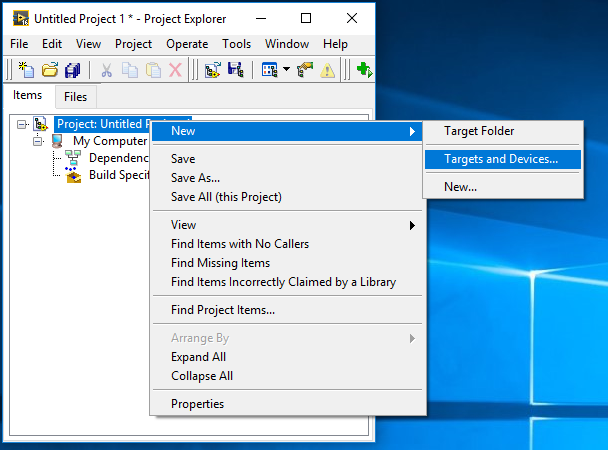
\includegraphics[scale=0.7]{figs/_1.png}
\caption{Add a new target to your project.}
\label{fig:_1}
\end{figure}

\begin{figure}[h!]
\hspace{40mm} 
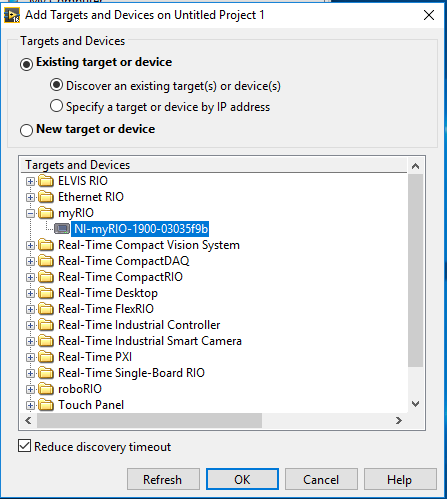
\includegraphics[scale=0.7]{figs/_2.png}
\caption{Add your myRIO to your project.}
\label{fig:_2}
\end{figure}

\begin{figure}[h!]
\hspace{25mm} 
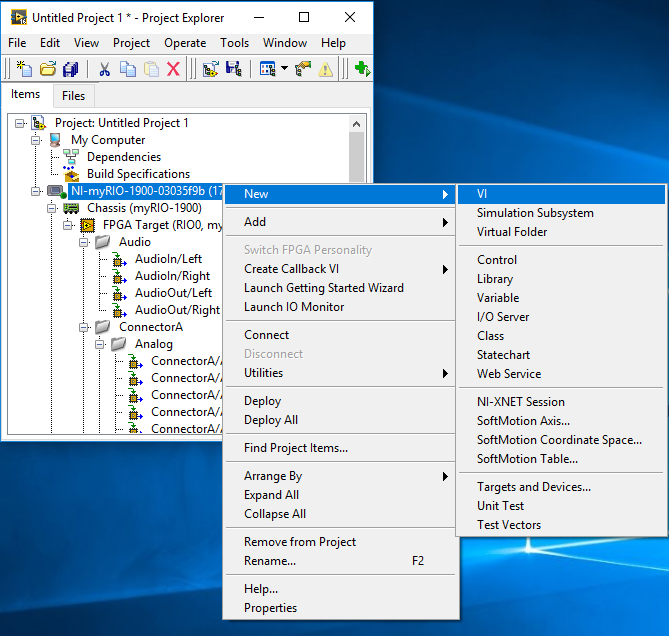
\includegraphics[scale=0.7]{figs/_3.png}
\caption{Add a VI to your myRIO.}
\label{fig:_3}
\end{figure}

\section{Programming with the accelerometer}
You need to build a VI which will read values from the built in accelerometer and plot them in real time. Your goal should (for now) should be to reconstruct the VI in Figure \ref{fig:_4}. In the structures pallet, select the flat frame sequence. In a flat frame sequence, all data to one of the frames must be ready before LabVIEW begins executing the subsequent frame. This structure is useful for programs that need initialization (actions that take place before the frame executes) and closing actions (actions that take place after the frame executes).

Next, create a while-loop and call it Main Loop. The While loop is available on the structures pallet. Put an instance of the Wait block in the while-loop and wire it with a constant 5 milliseconds. Feel free to play with this value. 

Then insert an express VI accelerometer from the myRIO pallet. Wire each of the axes to a bundle array block and feed the data to a waveform chart (the waveform chart is found in the front panel toolbox). Right click on the input error terminal and click on \textbf{Create}, then \textbf{Constant}. Drag the constant into the initialize frame and out of the while loop. Connect the output error terminal to an OR gate and the output of the OR gate to the while loop stop condition. The OR gate will also take a binary input from a button on the front panel. This will allow the program to stop if an error occurs or if the stop button is pressed. Also carry the error output outside of the while loop to the close frame. Wire it into a \textbf{Reset myRIO.vi} and then create an error out indicator. At this point, the front panel should look similar to the one in Figure \ref{fig:_5}. If your myRIO has been properly instantiated in your project, you should be able to run your code and observe the accelerometer waveforms.

If the board is not accelerating, it will experience 1g (in free fall, it would experience 0g. Please don’t try to test this!). The 1g vector always points upward with respect to the earth, no matter which way the board is rotated. This can be used to compute other useful data.

\section{Collecting data points}
It is important to be able to sample your signals and store those values into arrays for data processing purposes. In order to collect your data, you can add arrays to the border of your while loop. Simply connect your generated data wire to the border of the while loop, right click it and choose \textbf{Tunnel Mode: Indexing} to create an array which is automatically populated with a sample after each iteration of the while loop. You will need an array for each of your three data signals. Be sure to add some sort of front panel module which allows the user to view elements of the arrays. This can be done by adding an array module to the front panel and then dragging a numerical indicator into it. This should look something like Figure \ref{fig:array}.

\section{Elaborate on your data}
Your accelerometer produces 3 signals: X-axis, Y-axis, and Z-axis acceleration data. These signals can be used to compute the roll and pitch of your myRIO board. Use any equations or implementation methods you see fit to compute the roll and pitch of your board, and store those values into arrays corresponding to the same time samples as you did previously for the accelerometer data. For example, there should be 5 one-dimensional arrays which have $N$ values, where $N$ is the number of samples taken during the runtime of your code. Alternatively, you may construct a $5 \times N$ two-dimensional array that contains all your data. You should also have a second waveform chart on your front panel which plots the roll and pitch. 

You will also notice that your accelerometer data is very noisy. Build a simple low-pass filter using whatever method you prefer to smooth out your readings. The low-pass filter should be able to be turned off and have adjustable cutoff. 


\begin{figure}[h!]
\hspace{-20mm} 
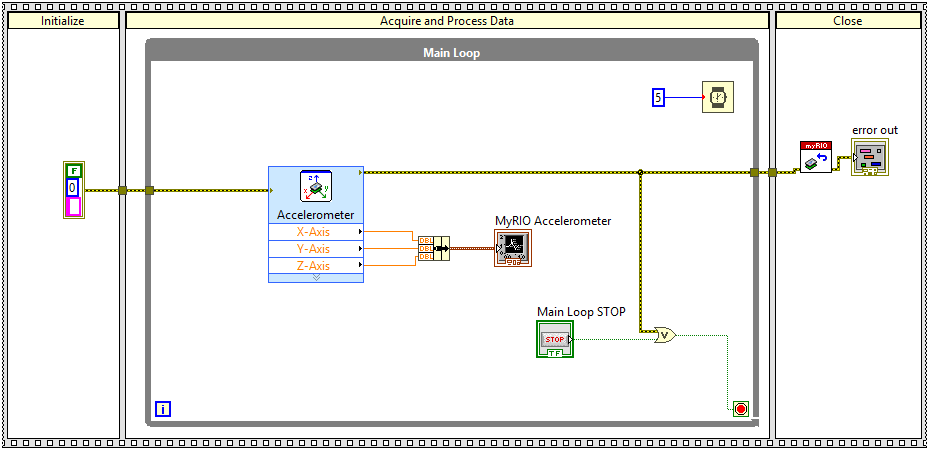
\includegraphics[scale=0.82]{figs/_4.png}
\caption{Block diagram.}
\label{fig:_4}
\end{figure}

\begin{figure}[h!]
\hspace{-20mm} 
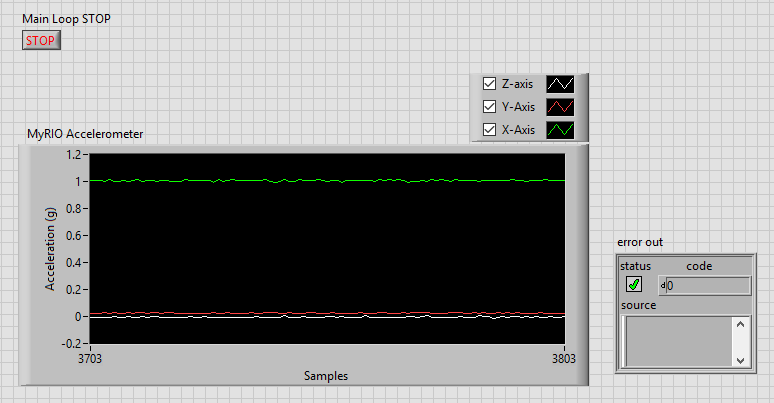
\includegraphics[scale=1]{figs/_5.png}
\caption{Front panel.}
\label{fig:_5}
\end{figure}

\begin{figure}[h!]
\hspace{25mm} 
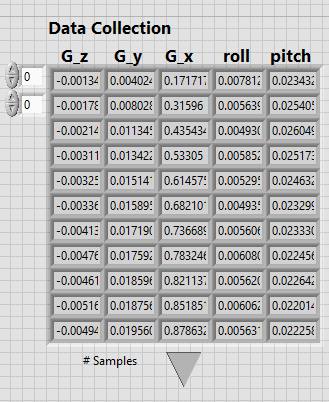
\includegraphics[scale=1]{figs/array.png}
\caption{Front panel array indicator module.}
\label{fig:array}
\end{figure}

\section{Submission requirements}

For this lab, you will be required to submit a .zip file containing your project file, your VI file, a screenshot of the final block diagram, and a screenshot of the final front panel in action. You will also be required to submit a URL to a private YouTube video with a maximum length of 90 seconds which demonstrates the full functionality of the accelerometer (as seen through the wavechart), your roll and pitch computation (also seen through a wavechart), your low-pass filter (must be able to turn it on/off and adjust cutoff point, effects should be visible in the wavecharts), and your data collection (arrays should be visibly populating during runtime).  

\end{document}
